\chapter{Security Considerations}
\label{chapter4}
\thispagestyle{empty}

\noindent Low Energy devices make of their efficient battery consumption their strong point; they support wireless technology and have an enormous range of applications. Manufacturers often prioritize the life-expectancy and battery life of the devices instead of their protection from external attacks. In Section \ref{sec:connection} we described the existing modes of communication and how to achieve pairing. A proper choice of the device and the association mode can mean much in terms of protection and security. In this chapter, we will explore this topic seeing also some concrete threats.

\section{BLE Threats}
We started our report by stating that we would study the fifth version of the specification, being the previous one made legacy. Nonetheless, as it happens, many new devices still implement Bluetooth connectivity 4.0, introducing a weakness in the protocol. In fact, the 5.0 Specification introduces a security upgrade called \textit{Secure Connections}. In this new protocol, the security level is raised both by sending challenges as well as using more complex cryptographic primitives for key generation. Secure Connections can sadly be established only when both devices implement them, otherwise they both switch to the previous version of the protocol.

In legacy systems, communications involve the exchange of a temporary key, which has subsequently been abandoned in favor of a more complex one. In general, it could be very important for an attacker to intercept the first packets of a communication, since many security parameters are then established. 
\subsection{Passive Eavesdropping}
As highlighted in this project, devices with a "Just Works" pairing mechanism do not offer any protection against passive attacks, which also happen to be quite straightforward. Sometimes it may also be possible to just intercept data from a device without being connected. Usually, no key is used to obfuscate the data, while if a key is present then it becomes important for the attacker to understand what it is at the beginning of the communication.
Differently, smart phones or  the tools analysed in the previous chapter such as \texttt{gatttool} or \texttt{bluetoothctl}, have no means of eavesdropping the exchanged data. However it may be possible with more sophisticated or ad hoc instruments like Ubertooth or Nordic Semiconductor Dongle, made specifically for the purpose of intercepting packets.
Another option to guarantee a superior level of security is using encrypted data in a way that ill-intentioned listeners are not able to decipher the messages sent.

\subsection{Man-In-The-Middle}
In this case the attacker first listens to the communication, then intercepts the messages sent from one device to the other. Before being delivered to the destination the message is modified. This security attack is also called \textit{Active Eavesdropping} due to the active role of the attacker, that remains invisible from the communicating devices. Even using a public key cryptography may not suffice against this kind of attack: if the attacker replaces the shared public key with its own public key, the attack will be successful.
In this context there are tools that allow users to try hands-on MITM attacks, like \texttt{btlejuice} or \texttt{gattacker}, that will be analysed more deeply in the next chapter.

\subsection{Identity Tracking}
BLE devices are often designed just to advertise data in a periodic way, updating their status or characteristics. However the packets contain the MAC address of the broadcaster and even information about the proximity of the device in terms of signal strength encoded in the RSSI field.
After gathering a comprehensive amount of data, and depending on the type of information the device advertises, it may be possible for the attacker to track the device, even more so if the data sent is specific for a certain entity (either a person or a device).

\subsection{Duplicate Device}
Man-In-The-Middle frameworks such as Btlejuice or Gattacker are also an example of another threat that may befall BLE devices: the creation of dummy devices. Once the MAC address is obtained, all the services and the characteristics are copied and then the dummy device is activated.

\section{Architecture}
BLE devices implement the key management and security manager on host instead of controller and all the key generation and distribution falls under its responsibility.
This approach is introduced by the Bluetooth Specification and helps the host to be flexible and reduces the cost and complexity of the controller.
The Security Manager defines the authentication, the pairing and encryption between the BLE devices and it uses the services provided by the L2CAP layer to manage all these functions.
\iffalse
\begin{figure}
	\centering	
	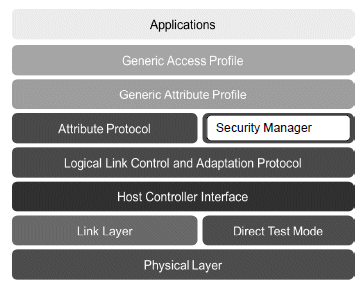
\includegraphics[width=0.5\textwidth]{architecture.gif}
	\label{fig:architecture}
\end{figure}
\fi
Security for BLE devices is expressed in LE Security Mode and may vary in a range from 1 to 4.
Each service and device may have a different security requirement.
\begin{itemize}
	\item LE Security Level 1: No secure communication and no pairing needed.
	\item LE Security Level 2: Support to authenticated and unauthenticated pairing but mandatory data signing with various techniques including public key cryptography.
	\item LE Security Level 3, 4: More security to the system than the other levels.
	\item Mixed Security Mode: There may be devices that need Level 1 and 2 and thus may use a combination of different security modes depending on the need.
	\item Secure Connection Only: Authenticated connection and pairing with encryption. Devices accept only outgoing and incoming connections for services that use security mode Level 4.
\end{itemize}

However, often BLE devices are weakly protected: few of them can use encryption while not requiring it (even the failed pairing is fine), and almost all devices are not strongly authenticated by mobile applications.
In addition to this BD address is often the only check needed to ensure authenticity. On the other side, as we will explain in the next chapter, attacks like sniffing and MITM are more difficult to accomplish than it seems.


